\documentclass[12pt,letterpaper]{article}
\usepackage[utf8]{inputenc}
\usepackage[spanish]{babel}
\usepackage{graphicx}
\usepackage[left=2cm,right=2cm,top=2cm,bottom=2cm]{geometry}
\usepackage{graphicx} % figuras
% \usepackage{subfigure} % subfiguras
\usepackage{float} % para usar [H]
\usepackage{amsmath}
%\usepackage{txfonts}
\usepackage{stackrel} 
\usepackage{multirow}
\usepackage{enumerate} % enumerados
\renewcommand{\labelitemi}{$-$}
\renewcommand{\labelitemii}{$\cdot$}
% \author{}
% \title{Caratula}
\begin{document}

% Fancy Header and Footer
% \usepackage{fancyhdr}
% \pagestyle{fancy}
% \cfoot{}
% \rfoot{\thepage}
%

% \usepackage[hidelinks]{hyperref} % CREA HYPERVINCULOS EN INDICE

% \author{}
\title{Caratula}

\begin{titlepage}
\begin{center}
\large{UNIVERSIDAD PRIVADA DE TACNA}\\
\vspace*{-0.025in}
\begin{figure}[htb]
\begin{center}

\includegraphics[width=8cm]{./Imagenes/logo}
\end{center}
\end{figure}
\vspace*{0.15in}
INGENIERIA DE SISTEMAS  \\

\vspace*{0.5in}
\begin{large}
TITULO:\\
\end{large}

\vspace*{0.1in}
\begin{Large}
\textbf{INFORME DE LABORATORIO No 01} \\
\end{Large}

\vspace*{0.3in}
\begin{Large}
\textbf{CURSO:} \\
\end{Large}

\vspace*{0.1in}
\begin{large}
BASE DE DATOS II\\
\end{large}

\vspace*{0.3in}
\begin{Large}
\textbf{DOCENTE(ING):} \\
\end{Large}

\vspace*{0.1in}
\begin{large}
 Patrick Cuadros Quiroga\\
\end{large}

\vspace*{0.2in}
\vspace*{0.1in}
\begin{large}
Estudiante: \\
\begin{flushleft}
Fiorella Rosmery Salamanca Contreras		\hfill	(2015053237) \\
\end{flushleft}
\end{large}
\end{center}

\vspace*{0.5in}
\begin{center}
\begin{large}
TACNA - PERU\\
2018
\end{large}
\end{center}

\end{titlepage}


\tableofcontents % INDICE
\thispagestyle{empty} % INDICE SIN NUMERO
\newpage
\setcounter{page}{1} % REINICIAR CONTADOR DE PAGINAS DESPUES DEL INDICE

\section{Actividad No 01 – Sistema Control de Versiones} 

\begin{itemize} % CREA GUIONES
\item \textbf{¿Que es un Sistema Control de Versiones?}\\

Un sistema de control de versiones (SCV) es una herramienta que nos permite el registro de todos los cambios hechos en uno o más proyectos, guardando así todas las versiones del producto en todas sus fases de desarrollo.
	
En un sistema control de versiones,las versiones son como fotografías que registran su estado actual en ese momento del tiempo y se van guardando a medida que se hacen modificaciones al código fuente.
	
Otros autores lo definen como un software que controla y organiza las
distintas revisiones que se realizen sobre uno o varios documentos,como los cambios realizados sobre un documento,
por ejemplo añadir un parrafo, borrar un fragmento o algo similar.\\

EJEMPLO:\\

En un principio se carga el siguiente codigo:\\

\begin{center}
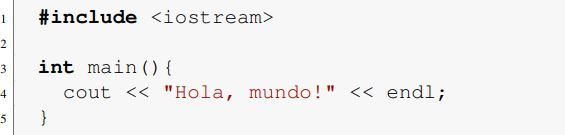
\includegraphics[width=12cm]{./Imagenes/actividad0101} 
\end{center}
	
Donde el SCV lo almacena como la version 1 del proyecto, de manera que si realizamos cambios se quedara almacenado por versiones.\\
	
Si quisieramos modificar el codigo por algún error que haya surgido,lo modificariamos de la siguiente manera:\\

\begin{center}
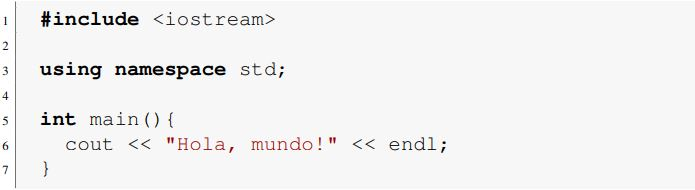
\includegraphics[width=13cm]{./Imagenes/actividad0102} 
\end{center}
	
Añadiendolo al SCV,este lo almacenara como la version 2 del proyecto,de manera que podamos tener todas las versiones de los cambios que se hayan hecho en el proyecto durante su tiempo de desarrollo.\\
\end{itemize} 


\begin{itemize}
\item \textbf{Caracteristicas de un Sistema Control de Versiones:} \\

Un sistema de control de versiones debe proporcionar:\\

\begin{enumerate}[1.] % CREA ENUMERACION
\item Mecanismo de almacenamiento de los elementos que deba gestionar.
\item Posibilidad de realizar cambios sobre los elementos almacenados.
\item Registro histórico de las acciones realizadas con cada elemento o conjunto de elementos.\\
\end{enumerate}
\end{itemize} 


\begin{itemize}
\item \textbf{Clasificacion de un Sistema Control de Versiones:} \\

Los sistemas de control de versiones se pueden clasifica en 2 grandes grupos:\\

\begin{enumerate}[1.] % CREA ENUMERACION
\item Centralizados\\

En un sistema de control de versiones centralizado todos nuestros fuentes y sus versiones están almacenados en un único directorio de un ordenador. Todos los desarrolladores que quieran trabajar con esos fuentes, deben pedirle al sistema de control de versiones una copia local para trabajar. En ella realizan todos sus cambios y cuando están listos y funcionando, le dicen al sistema de control de versiones que guarde los fuentes modificados como una nueva versión.\\

\item Distribuidos\\

En un sistema de control de versiones distribuido no hay un repositorio central. Todos los desarrolladores tienen su propia copia del repositorio, con todas las versiones y toda la historia. Según van desarrollando y haciendo cambios, sus fuentes y versiones van siendo distintas unas de otras.\\
\end{enumerate}
\end{itemize} 


\begin{itemize}
\item \textbf{Funcionamiento de un Sistema Control de Versiones:} \\

Todos los sistemas de control de versiones se basan en disponer de un repositorio, que es el conjunto de información gestionada por el sistema. Este repositorio contiene el historial de versiones de todos los elementos gestionados.

Cada uno de los usuarios puede crearse una copia local duplicando el contenido del repositorio para permitir su uso. Para modificar la copia local existen dos semánticas básicas:\\

\begin{enumerate}[1.] % CREA ENUMERACION
\item Exclusivos

Para poder realizar un cambio es necesario marcar en el repositorio el elemento que se desea modificar y el sistema se encargará de impedir que otro usuario pueda modificar dicho elemento.\\

\item Colaborativos

En el que cada usuario se descarga la copia, la modifica, y el sistema automáticamente combina las diversas modificaciones. Puede estar sujeto a la aparición de conflictos que deben ser solucionados manualmente.\\
\end{enumerate}
\end{itemize} 


\section{Actividad No 02 – Sistema de Control de Versiones Libres} 
Entre los sistemas de control de versiones que estan disponibles de manera libre tenemos los siguientes:

\begin{enumerate}[1.]

\item \textbf{CVS:} \\

El Concurrent Versions System (también conocido como Concurrent Versioning System) es una aplicación informática bajo licencia GPL que implementa un sistema de control de versiones.

Se encarga de mantener el registro de todo el trabajo y los cambios en los ficheros (código fuente principalmente) que conforman un proyecto y permite que distintos desarrolladores (potencialmente situados a gran distancia) colaboren.\\

\item \textbf{Subversion:} \\

SVN es conocido así por ser el nombre del cliente, el software en sí es llamado SUBVERSION.

SUBVERSION es un sistema centralizado para compartir información que fue diseñado como reemplazo de CVS.

La parte principal de SUBVERSION es el repositorio, el cual es un almacén central de datos. El repositorio guarda información en forma de árbol de archivos. .\\

\item \textbf{SVK:} \\

Aunque se ha construido sobre Subversion, probablemente SVK se parece más a algunos de los anteriores sistemas descentralizados que a Subversión. 

SVK soporta desarrollo distribuido, cambios locales, mezcla sofisticada de cambios, y la habilidad de "reflejar/clonar" árboles desde sistemas de control de versiones que no son SVK.\\

\item \textbf{Mercurial:} \\

MERCURIAL es otro sistema de control de versiones muy extendido, el creador y desarrollador principal de MERCURIAL es Matt Mackall. Está implementado principalmente haciendo uso del lenguaje de programación Python, pero incluye una implementación binaria de diff escrita en C.\\

\item \textbf{GIT:} \\

GIT es uno de los sistemas de control de versiones distribuidos más usados. Fue creado por Linus Torvalds1 y buscaba un sistema que cumpliera 4 requisitos básicos:

-No parecido a CVS
-Distribuido
-Seguridad frente a corrupción, accidental o intencionada
-Gran rendimiento en las operaciones

GIT está escrito en C y en gran parte fue construido para trabajar en el kernel de Linux, lo que quiere decir que desde el primer día ha tenido que mover de manera efectiva repositorios de gran tamaño.\\

\item \textbf{Bazaar:} \\

Bazaar está todavía en desarrollo. Será una implementación del protocolo GNU Arch, mantendrá compatibilidad con el procotolo GNU Arch a medida que evolucione, y trabajará con el proceso de la comunidad GNU Arch para cualquier cambio de protocolo que fuera requerido a favor del agrado del usuario.\\

\end{enumerate}



\section{Actividad No 03 – Herramientas Similares al GitHub} 
		
\begin{itemize} % CREA GUIONES
\item \textbf{¿Que es GitHub?}\\

GitHub es un servicio de alojamiento web para proyectos que utilizan el sistema de control de revisiones Pequeño icono de GitGit . Está escrito en Ruby on Rails por los desarrolladores de Logical Awesome Chris Wanstrath, PJ Hyett y Tom Preston-Werner. GitHub ofrece planes comerciales y cuentas gratuitas para proyectos de código abierto.

El sitio proporciona funciones de redes sociales como una alimentacion de contenido, seguidores y el gráfico de red para mostrar cómo los desarrolladores trabajan en sus versiones de un repositorio.

Otros autores lo señalan como una plataforma de desarrollo colaborativo de software para alojar proyectos utilizando el sistema de control de versiones Git,debido a que el código se almacena de forma pública, aunque también se puede hacer de forma privada, creando una cuenta de pago.\\

\begin{center}

\includegraphics[width=6cm]{./Imagenes/actividad0301} 
\end{center}
	
\end{itemize} 


\begin{itemize} % CREA GUIONES
\item \textbf{¿Porque es importante GitHub?}\\

GitHub permite alojar en tu repositorio el código de desarrollo de proyecto y te brinda herramientas muy útiles para el trabajo en equipo, dentro de un proyecto.

Además de eso, puedes contribuir a mejorar el software de los demás. Para poder alcanzar esta meta, GitHub provee de funcionalidades para hacer un fork y solicitar pulls.

Realizar un fork es simplemente clonar un repositorio ajeno (genera una copia en tu cuenta), para eliminar algún bug o modificar cosas de él. Una vez realizadas tus modificaciones puedes enviar un pull al dueño del proyecto. Éste podrá analizar los cambios que has realizado fácilmente, y si considera interesante tu contribución, adjuntarlo con el repositorio original.\\

\begin{center}
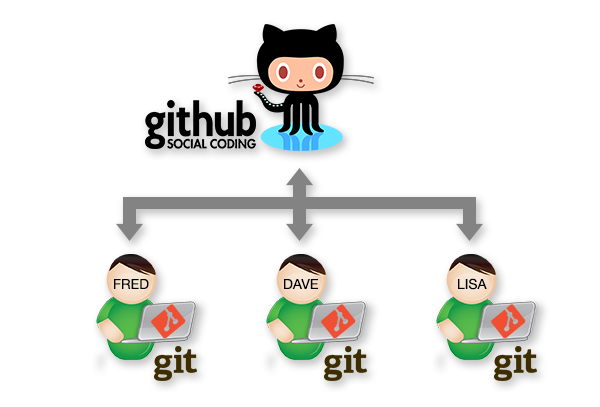
\includegraphics[width=12cm]{./Imagenes/actividad0302} 
\end{center}
	
\end{itemize} 


\begin{itemize} % CREA GUIONES
\item \textbf{¿Qué herramientas proporciona?}\\

En la actualidad, GitHub es mucho más que un servicio de alojamiento de código. Además de éste, se ofrecen varias herramientas útiles para el trabajo en equipo. Entre ellas, caben destacar:

\begin{enumerate}[1.]

\item Una wiki para el mantenimiento de las distintas versiones de las páginas.\\

\item Un sistema de seguimiento de problemas que permiten a los miembros de tu equipo detallar un problema con tu software o una sugerencia que deseen hacer.\\

\item Una herramienta de revisión de código, donde se pueden añadir anotaciones en cualquier punto de un fichero y debatir sobre determinados cambios realizados en un commit específico.\\

\item Un visor de ramas donde se pueden comparar los progresos realizados en las distintas ramas de nuestro repositorio.\\

\end{enumerate}	
\end{itemize} 

\begin{itemize} % CREA GUIONES
\item \textbf{Herramientas Similares al GitHub}\\

A pesar de que GitHub sea la plataforma más utilizada para almacenar proyectos basados en código abierto en Internet, existen otras opciones que se puede elegir para publicar y almacenar en la nube nuestros proyectos,entre los cuales tenemos:

\begin{enumerate}[1.]

\item Bitbucket\\

Bitbucket se trata de otra plataforma muy popular en la que individuos y organizaciones tienden a almacenar sus repositorios basados en código libre. 

Permite tener repositorios públicos, como así también privados ilimitados, lo cual atrae la atención de los desarrolladores que acostumbran a necesitar espacio de almacenamiento para almacenar sus archivos en la nube.

\begin{center}
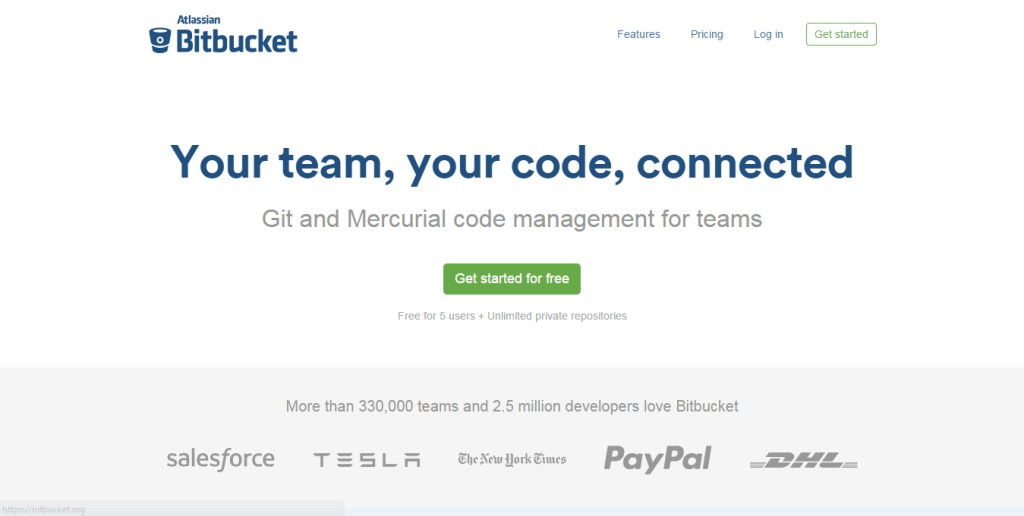
\includegraphics[width=12cm]{./Imagenes/actividad0303} 
\end{center}

\item SourceForge\\

SourceForge es otra reconocida página web en el que desarrolladores acostumbran a publicar sus proyectos basados en diferentes plataformas y compatibles con los más variados sistemas operativos, como Linux, Windows y Mac. 

Una de las particularidades de SourceForge es que permite únicamente crear proyectos de código abierto con nombre único, por lo que deberemos ser originales al momento de publicar nuestras creaciones. 

\begin{center}
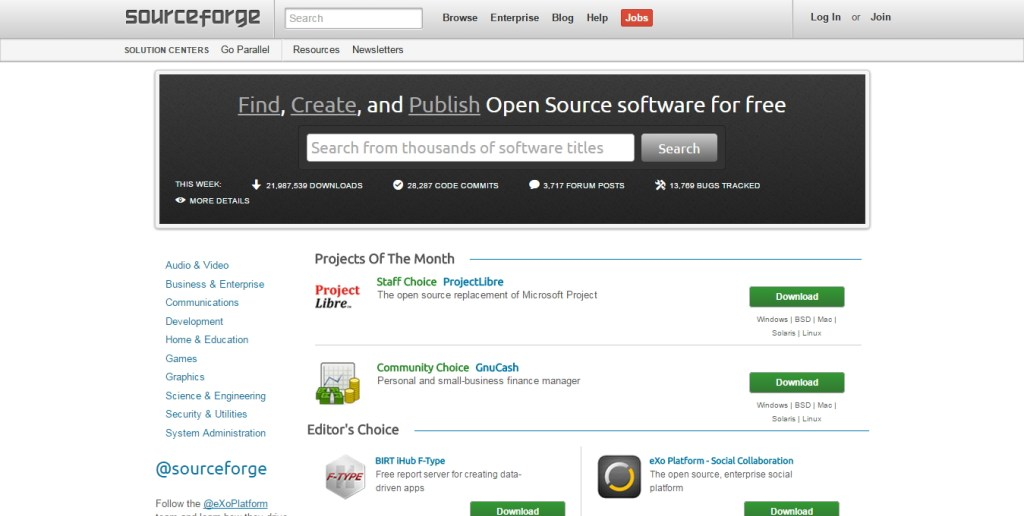
\includegraphics[width=12cm]{./Imagenes/actividad0304} 
\end{center}

\item GitLab\\

GitLab es una página web similar, aunque en este caso destaca la posibilidad de permitirle a sus usuarios instalar esta plataforma en sus servidores particulares, lo cual permite no tan solo que el usuario pueda asociar un dominio personal a su cuenta de GitLab, sino que también puede asociar un servidor web propio, lo cual le permitirá gozar de mayor seguridad y privacidad en los contenidos.

\begin{center}
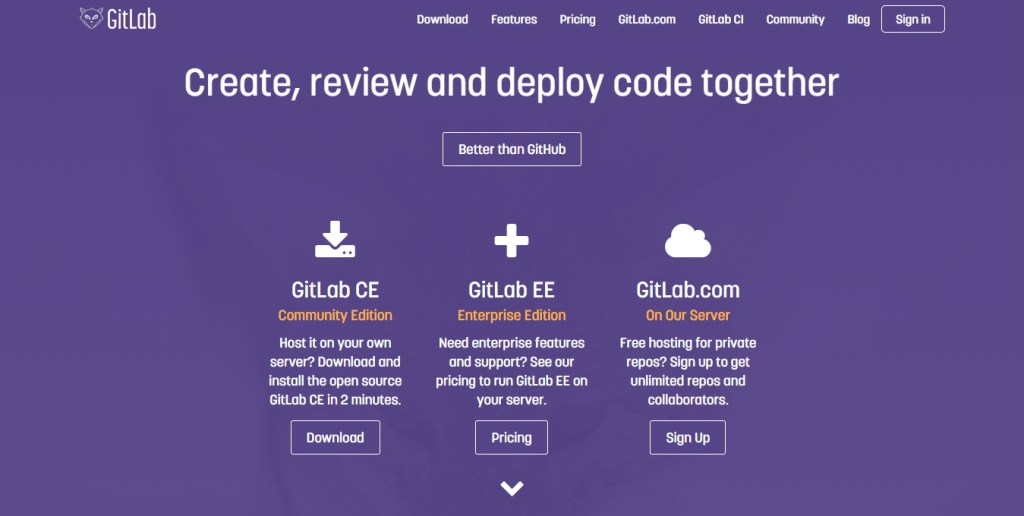
\includegraphics[width=12cm]{./Imagenes/actividad0305} 
\end{center}

\item Kiln\\

El host Kiln es una opción de pago que ofrece mejores servicios. 
Al contratar un plan dentro de este host conseguiremos obtener de manera gratuita un subdominio para nuestra empresa, desde el cual podremos almacenar todos nuestros proyectos en una página web particular.

\begin{center}
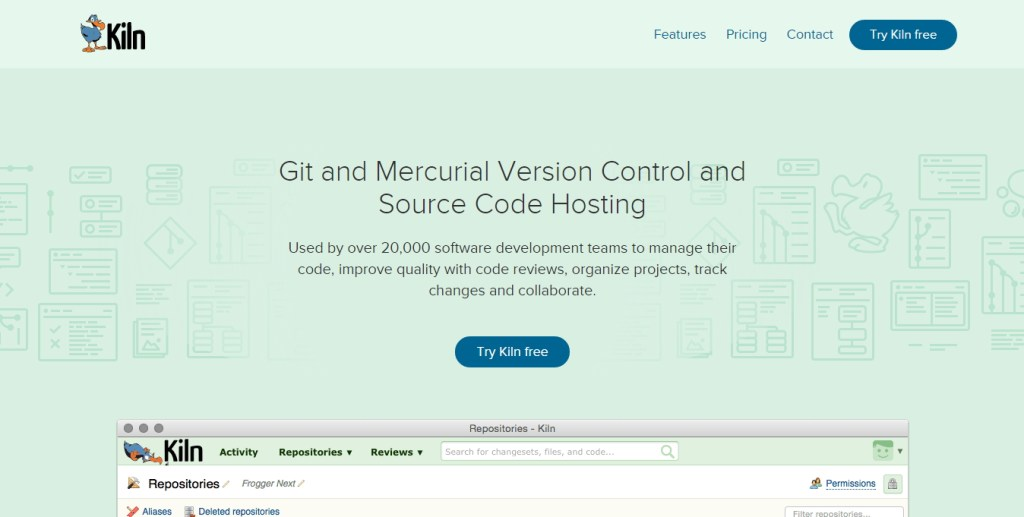
\includegraphics[width=12cm]{./Imagenes/actividad0306} 
\end{center}

\item Codeplane\\

Codeplane es otro servicio de pago, a través del cual podremos almacenar nuestros proyectos en Internet. 
También dentro de este servicio tenemos herramientas como es el caso de la copia de seguridad de los repositorios, y las posibilidades de publicación de proyectos.

\begin{center}
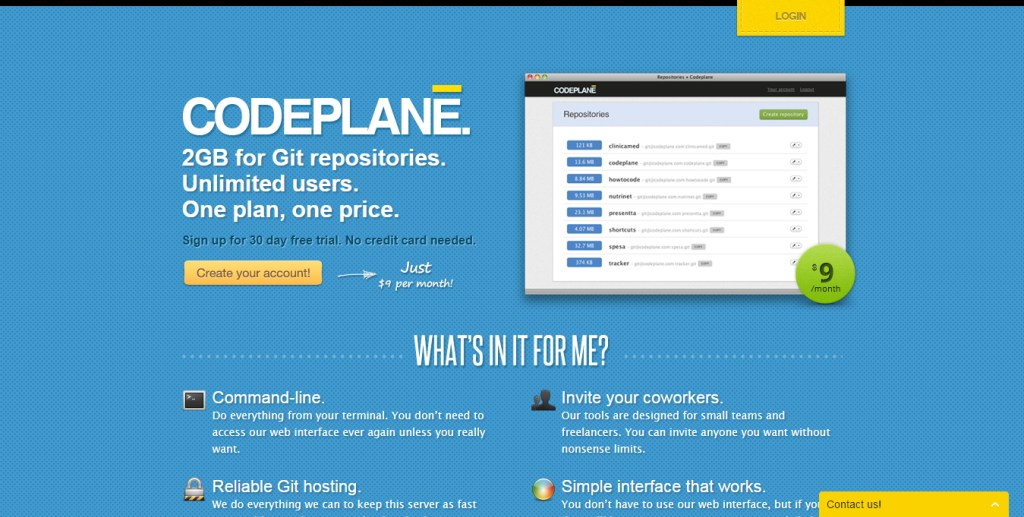
\includegraphics[width=12cm]{./Imagenes/actividad0307} 
\end{center}

\item CodePlex\\

Microsoft nos ofrece un servicio gratuito de almacenamiento de código fuente llamado CodePlex, el cual nos permite crear proyectos e incluso tener nuestro propio sitio con subdominio.

Para publicar proyectos necesitaremos hacerlo con títulos únicos, ya que al igual que SourceForge, CodePlex no nos permite realizar publicaciones con el mismo nombre para buscar originalidad en los proyectos.

\begin{center}
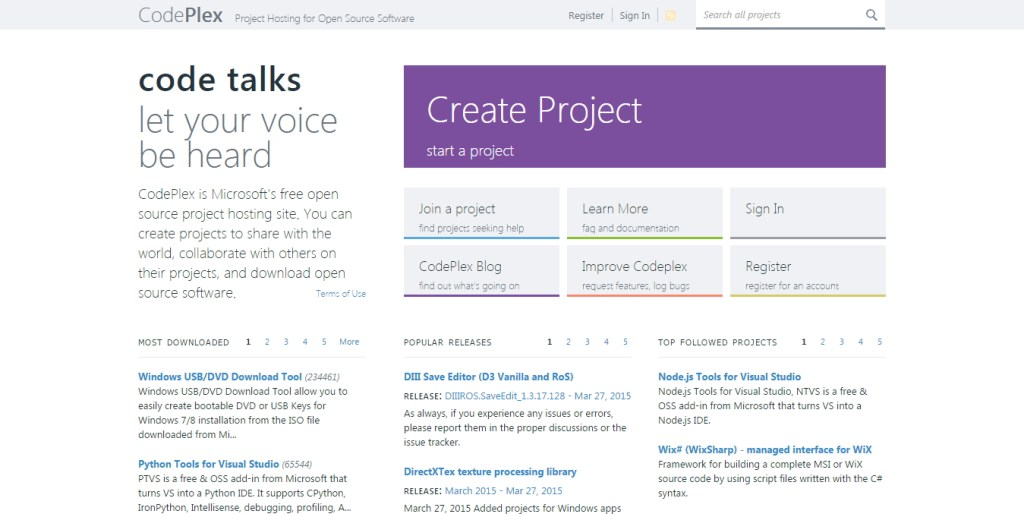
\includegraphics[width=12cm]{./Imagenes/actividad0308} 
\end{center}

\item Beanstalk\\

Beanstalk es una plataforma premium que nos ofrece cuentas gratuitas por dos semanas para probar el alcance de cada función que incluye. No necesitaremos herramientas adicionales, ya que al igual que GitHub, podremos editar el código desde nuestro navegador web.

\begin{center}
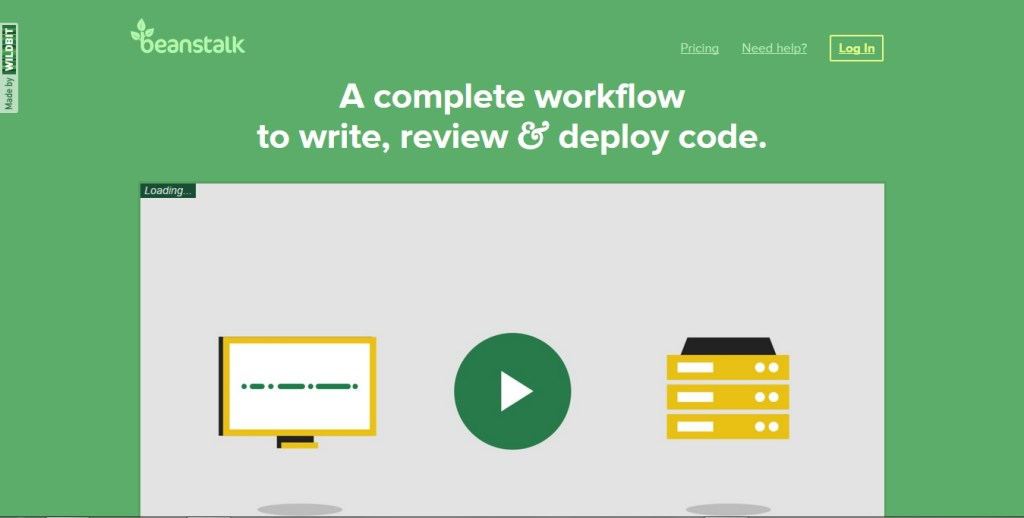
\includegraphics[width=12cm]{./Imagenes/actividad0309} 
\end{center}

\end{enumerate}

\end{itemize} 






\end{document}
